% \documentclass[journal]{IEEEtran}
\documentclass[12pt,journal,draftclsnofoot,onecolumn]{IEEEtran}
\IEEEoverridecommandlockouts

% remove colon after subsubsection, use spacing instead
\makeatletter
\renewcommand{\@IEEEsectpunct}{\quad}
\makeatother

\makeatletter
% add a small spacing *before* subsections
\let\origsubsubsection\subsubsection
\renewcommand\subsubsection{\@ifstar{\starsubsubsection}{\nostarsubsubsection}}

\newcommand\nostarsubsubsection[1]
{\subsubsectionprelude\origsubsubsection{#1}}

\newcommand\subsubsectionprelude{%
  \vspace{6pt}
}
\makeatother

% change default font to charter
% \usepackage{charter}
% \usepackage[bitstream-charter]{mathdesign}
% \usepackage{XCharter}
\usepackage{amsfonts}

% Fixing IEEEtran.cls bug with [english]{babel}
\makeatletter
\def\markboth#1#2{\def\leftmark{\@IEEEcompsoconly{\sffamily}\MakeUppercase{\protect#1}}%
\def\rightmark{\@IEEEcompsoconly{\sffamily}\MakeUppercase{\protect#2}}}
\makeatother

% \usepackage{t1enc}

\usepackage{listings}
\usepackage{multirow}
%\usepackage[utf8x]{inputenc}
\usepackage[english]{babel}
\selectlanguage{english}
\usepackage{color}
%\usepackage{caption}
\usepackage{cite}
\usepackage[pdftex]{graphicx}

% \usepackage{subfig}
\usepackage{subcaption}
\usepackage{amsmath}

\usepackage{mathtools}
\DeclarePairedDelimiter\ceil{\lceil}{\rceil}
\DeclarePairedDelimiter\floor{\lfloor}{\rfloor}

\usepackage{amsfonts}
\usepackage{array}
\usepackage{verbatim}
\usepackage{listings}
\usepackage[hidelinks]{hyperref}
\usepackage{url}
\usepackage{enumerate}
\usepackage{multirow}

\usepackage{siunitx}
\usepackage{epsfig}
\usepackage{epstopdf}
\usepackage{multicol}% http://ctan.org/pkg/multicols
\usepackage[font=footnotesize]{caption}
% \usepackage[font=scriptsize]{subcaption}
% Tikz
\usepackage{tikz}
\usepackage{pgfplots}
\pgfplotsset{compat=newest}
\pgfplotsset{plot coordinates/math parser=false}
\newlength\fheight
\newlength\fwidth
\usetikzlibrary{patterns,decorations.pathreplacing,backgrounds,calc}
\definecolor{SchoolColor}{RGB}{0.71, 0, 0.106}%181,0,27} unipd red
\definecolor{chaptergrey}{rgb}{0.61, 0, 0.09} % dialed back a little
\definecolor{midgrey}{rgb}{0.4, 0.4, 0.4}
\definecolor{chaptergreen}{rgb}{0.09, 0.612, 0}
\definecolor{chapterpurple}{rgb}{0.522, 0, 0.612}
\definecolor{chapterlightgreen}{rgb}{0, 0.612, 0.522}

%\raggedbottom

% Pseudocode
\usepackage[ruled, vlined]{algorithm2e}

\SetKwRepeat{Do}{do}{while}
\SetKwBlock{wpPa}{with probability $P_A$}{end}
\DontPrintSemicolon
% \usepackage{algorithm}
% \usepackage[noend]{algpseudocode}
% \renewcommand\algorithmicthen{}
% \renewcommand\algorithmicdo{}
\usepackage{lscape}

\addto\captionsenglish{\renewcommand{\figurename}{Fig.}}

\newcommand{\field}[1]{\mathbb{#1}}

\DeclareMathOperator*{\argmin}{arg\,min}
\DeclareMathOperator*{\argmax}{arg\,max}
\newcommand{\norm}[1]{\left\lVert#1\right\rVert}
\renewcommand{\arraystretch}{2}

\newcommand{\DP}[1]{\textcolor{blue}{\textbf{(DP says: #1)}}}
\newcommand{\cri}[1]{\textcolor{violet}{\textbf{(Cri says: #1)}}}

\usepackage{threeparttable}
%\usepackage[table,xcdraw]{xcolor}
\usepackage{tabularx}
\usepackage{multirow}
\usepackage{booktabs}
\newcommand{\tabitem}{~~\llap{\textbullet}~~}
\usepackage{array, blindtext}
\usepackage{wrapfig}
\usepackage{pdfpages}
\usepackage[acronym]{glossaries}

% use tikArchiviz images or eps
\newif\iftikz
\tikztrue

\graphicspath{{./figures/}}

\title{Technology-based aids for people affected by Autism Spectrum Disorder (ASD)}
\author{\IEEEauthorblockN{Cristina Gava, Peron Davide}\\
\small{{Neurosensorial Engineering final project\\
A.A. 2017/2018\\}}
}

% Reduce the space below figs.
%\setlength{\belowcaptionskip}{-0.7cm}

\renewcommand{\equationautorefname}{Eq.}

%% Glossary
\newacronym{asd}{ASD}{Autism Spectrum Disorder}
\newacronym{va}{VA}{Virtual Agents}
\newacronym{dof}{DoF}{Degrees of Freedom}

\glsresetall
\begin{document}

\def\equationautorefname~#1\null{(#1)\null}
\setlength{\belowcaptionskip}{-0.2cm}

% reduce space after title
\makeatletter
\patchcmd{\@maketitle}
  {\addvspace{0.5\baselineskip}\egroup}
  {\addvspace{-1.2\baselineskip}\egroup}
  {}
  {}
\makeatother

\maketitle

\begin{abstract}
Individuals affected by Autism Spectrum Disorder(ASD), especially the not-verbal ones, are often unable to communicate in an
appropriate way, they show strong difficulties in social interactions and in manifesting their affective
states or their necessities.
The conventional techniques, used to improve the performances of these people in the
everyday tasks, are observation-based and can require a lot of effort in terms of time and money, with limited
results.
Technology-assisted therapies can result more powerful and fast.

Our aim is to analyze the current technology-based solutions that can help the therapist and the family of an autistic subject to interact with him.
These solutions exploit the joint use of human intelligence and artificial intelligence to improve
the powerfulness of therapies and to allow a better integration of these individuals in the society.
\end{abstract}
\begin{IEEEkeywords}
\centering
Autism Spectrum Disorder, Avatar-robots, Wearable Technology, Health Monitoring
\end{IEEEkeywords}
\clearpage

\tableofcontents
\clearpage

\glsresetall
\section{Introduction} \label{sec:introduction}

% TODO Brief presentation of ASD (?)
\gls{asd} is a term used to cover a very big set of disorders. In this field there are a lot of studies and experiments, but still is one of the most unknown \DP{forse unknown non è il massimo come termine qui} disease. The symptoms are well known, while the causes are mostly unknown. Nowadays, \textit{screening tests} are used to classify a person as affected by \gls{asd}, but these tests have an high percentage of error (false positive or negative) and they can be administered on a patient at least 3 years old. For this reason, several techniques have been studied to wonder if a children has this disorder in the first 2 years of life.

In this respect, this work is divided in two main sections. In \autoref{sec:thera_tech} we present some innovative tool to improve social skills of a child affected by ASD faster than a classical face-to-face therapy will does \DP{Questa frase fa schifo}.
In \autoref{sec:every_tech} we present a couple of wearable products that allow a faster and easier integration of the subject in the everydays tasks.

\section{Therapeutical techniques}
\label{sec:thera_tech}

The classical way to conduct a therapy session, is a face-to-face meeting between the subject and the therapist.
Usually, is conducted in four phases: the first one is called \textit{Instruction}, in which the therapist explain what is the skill that the subject is going to learn; the second one is the \textit{Modeling} phase, in which the therapist show the patient what he has to do; there is then the \textit{Rehearsal} phase, in which the patient tries to imitate the therapist and finally a \textit{Feedback} phase in which the therapist draw its own conclusions about the test.
The problem of this kind of therapy are the completely subjective evaluation procedure carried out by the therapist and that the subject's attention is not immediate.

%TODO Avatar-based techniques to improve the performances of the therapy
%TODO Methods to detect the anxiety level
To improve the performances of the sessions, the use of \gls{va} platforms has been introducted.
A \gls{va} platform consist of an avatar, that can be a robot or a virtual character, a learning software that receives information from the Avatar, elaborates them and adjusts the response of the Avatar, and an interface for the therapist to interpretate the results.
In a \gls{va} session, the therapist, with the aids of the learning software, learns the Avatar in order to do an action that the child has to imitate, the child tries to imitate the Avatar, learning new way to interact with the society.

Different system has been proposed, we propose here two different solutions, one more general and one more complex and efficient.

\subsection{General AVATAR idea}
\label{sec:avatar_general}

\begin{figure}[h]
\centering

\begin{minipage}{0.48\textwidth}
\centering
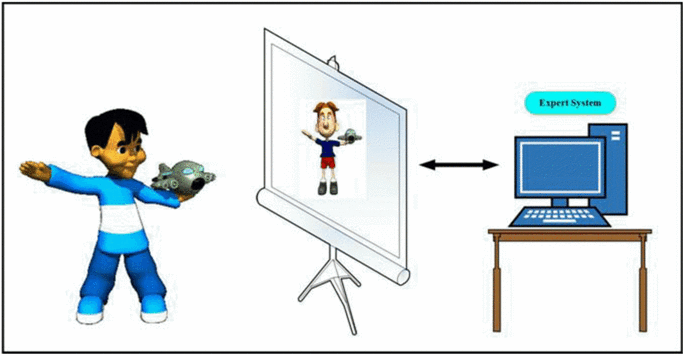
\includegraphics[width=\textwidth]{avatar_system.png}
\caption{Scheme of AVATAR system}
\label{fig:avatar_scheme}
\end{minipage}
\begin{minipage}{0.48\textwidth}
\centering
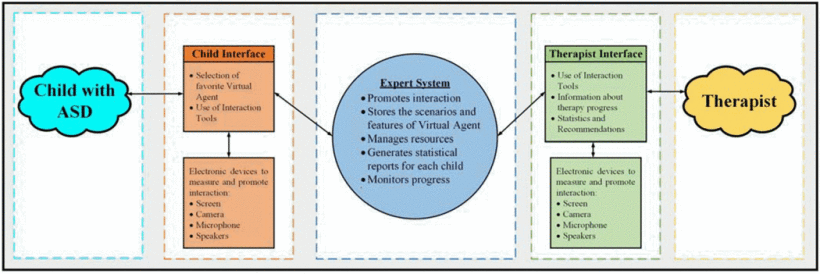
\includegraphics[width=\textwidth]{avatar_tasks.png}
\caption{Structure of AVATAR platform}
\label{fig:avatar_tasks}
\end{minipage}

\end{figure}

The idea of an Avatar-based therapy session is proposed firstly in \cite{Guerrero-vasquez}. They propose a system composed by a \gls{va} and an \textit{expert system} used by the therapist to instruct the \gls{va}. A general scheme of the proposed system is shown in \autoref{fig:avatar_scheme}.

They chose to use a \gls{va} instead of a robot since, according with the needs, it provides the possibility to customize the tools it offers and its appearance, while a robot is limitated on its shape and its \gls{dof}.

As can be seen in \autoref{fig:avatar_tasks}, the platform is organized as follow:
\begin{LaTeXdescription}
	\item[Child Interface] It selects the child's favourite \gls{va} and uses interaction tools as screen, camera, microphone and speakers to interact with the child;
	\item[Expert System] Contains a learning algorithm that promotes interaction between the child and the \gls{va}, it stores the scenario and features of the chosen \gls{va} and it monitors progress of the session in order to generate statistical reports that will be used by the therapist;
	\item[Therapist Interface] Allow the therapist to access to the reports generated by the Expert System and gives information about the current therapy, in order to allow the therapist to draw conclusions.
\end{LaTeXdescription}

The choices about the best \gls{va} to use during the sessions, or the characteristics that has to be changed in the current \gls{va}, are taken monitoring the reaction of the child when he's put in front of one of them.
The character can be not strictly a human, since the highest degree of affinity can be towards an animal or an object.

The key point in their work is that the information received on the screen of the Therapist Interface shows a real time image of the child and the monitored progress statistics.
Since the \gls{va} that the child observes on his screen is a disguise of his therapist, combined with artificial intelligence, is actually the therapist in combination with the expert system who promotes the interaction.

\subsection{A more complex system}
\label{sec:avatar_complex}

Another more complex and complete approach was performed in \cite{Alahbabi17}, using a robot instead of a \gls{va}, since it has been shown in \cite{Pioggia08} that patients show a more favorable response towards humanoid robots than to other non-humanoid virtual characters.

This approach has sensible advantages but also some intrinsic shortcomings:
\begin{itemize}
	\item most of the robotic or virtualized therapies are pre-programmed, that make the session boring and repetitive;
	\item robots are limited and work in a controlled environment;
	\item usually robots don't have a quantitative behavioral analysis tool due to the absence of therapists during their development process.
\end{itemize}

In this work they try to fulfill these lacks using a set of advanced technology tools, specifically a \textit{NAO Robot} (visible in \autoref{fig:nao_robot}) and a Perception Neuron Set of 32 sensors.

In their proposal, the robot will replace the therapist in the room.
The therapist would wear portable motion sensors giving him a partial control of the robot motion, and he would receive a visual and auditory stream from the robot. The therapist would also be able to talk to the child through the robot, by using a robotic voice.

\begin{figure}[h]
\centering

\begin{minipage}{0.48\textwidth}
\centering
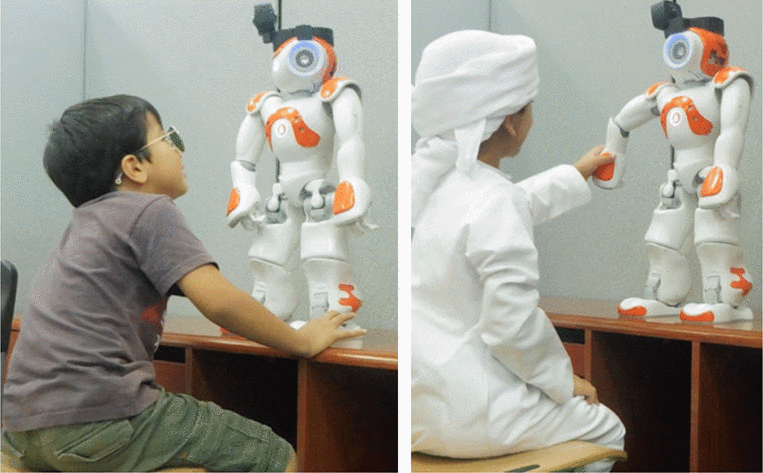
\includegraphics[width=\textwidth]{nao_robot.png}
\caption{Scheme of AVATAR system}
\label{fig:nao_robot}
\end{minipage}
\begin{minipage}{0.48\textwidth}
\centering
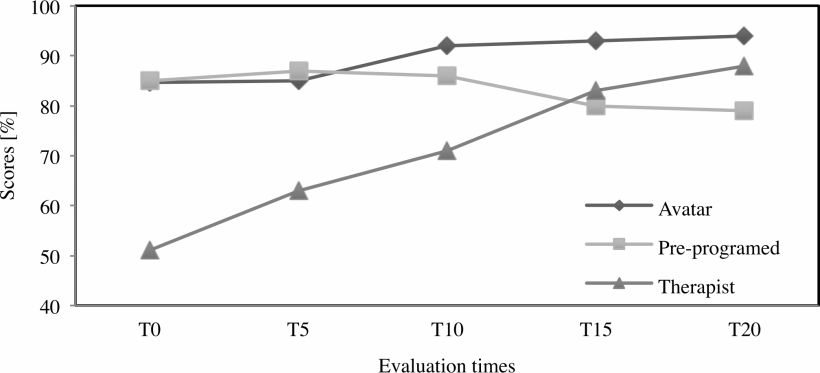
\includegraphics[width=\textwidth]{scores.png}
\caption{Structure of AVATAR platform}
\label{fig:scores}
\end{minipage}

\end{figure}

The strength of this work is that the robot behavior can be adapted based on the degree of engagement of the child in the session.
Indeed, as the session starts, a low number of \gls{dof} are given to the robot, in order to makes the child imitate a set of very simple movements.
As the patient progresses in the engagement (we'll see later that this means take more points), more \gls{dof} are given to the robot, usually enabling disabled actuators, in order to increase the complexity of the movements.

During the whole process a heart-rate measuring band is worn by the partecipant, to monitor the partecipant's level of anxiety and stop or change the session whenever an intervention is required.

To monitor the actual movements performed by the child, a Microsoft Kinect is used.

The movements performed by the robot and imitated by the child are specifically selected to teach the child how to interact with other people and to improve his response to social stimolous.

During the session, points are given to the child as he progresses and performs the right movement at the right time.
The total score is given by the sum of three contributes:

\begin{LaTeXdescription}
	\item[Motion Score] Is relative to the goodness of the movement made by the patient to imitate the robot;
	\item[Attention Score] the child takes one point for each second he's looking at the robot’s face whenever the robot is asking him a question;
	\item[Response Score] for this score, points are given for the delay time between the moment in which the robot asks a question and moment in which the child start answering the questions.
	10 points are given for the first 10 seconds after the robot/therapist stops talking, and one point is subtracted for each second of delay.
\end{LaTeXdescription}

After 20 minutes of session therapy, results are collected.
This experiment has been done in five healthy male children and with three different type of interaction subject: an avatar programmed as said before, a pre-programmed robot and a therapist in a classical face-to-face session. Score has been collected for each type of interaction and the results are shown in \autoref{fig:scores}.

As we can see the performance of the avatar are initially almost equal to the ones of a pre-programmed robot, but along the session, child gets bored of the last one due to its repetitive movements and requirements, while the score with the avatar increases due to its continuous adaption to the child needs.
The scores collected with a real therapist are very lower at the beginning compared with the first two type of interaction and it increases along the session since the therapist adapts the requirements to the child needs.

\section{Everydays tools techniques}
\label{sec:every_tech}

\subsection{Jumping Ball}
\subsection{Genetic Algorithm}

\section{Conclusions}\label{sec:conclusions}

\bibliographystyle{IEEEtran}
\bibliography{IEEEabrv,bibliography}

\end{document}
